\documentclass[../slides.tex]{subfiles}

\title{2018-2019 Inleiding Logica (KI1V13001) \\ Lecture 5}
 
\date{September 24, 2019\\[2ex] {\tiny \textcopyright~The non-copyrighted content of these slides is open access under \href{https://creativecommons.org/licenses/by-sa/4.0/}{CC BY-SA 4.0}}}
 
%%%%%%%%%%%%%%%

\begin{document}

\setcounter{framenumber}{128}
\begin{frame}
	\maketitle
\end{frame}

\begin{frame}{Overview}
\tableofcontents
\end{frame}

\section{Rehash}
\begin{frame}{Rehash}
	
 \begin{itemize}

	\item A formal language is defined by a vocabulary (symbols) and a grammar (rules).
	
	\item The vocabulary of a propositional language consists of $\mathcal{P}$ and $\neg,\land,\lor,\to,\leftrightarrow$.
	
	\item \alert{The set $\mathcal{L}$ of formulas is the smallest set containing the sentence letters and is closed under the connectives.} 
	
	\item Formalization is the process of abstracting ordinary language expressions into a propositional language.
	
	\item \alert{For syntactic recursion you specify the values the $\mathcal{P}$'s and how $\neg,\land,\lor,\to,\leftrightarrow$ affect the value.}
	
	\item \alert{The parsing tree shows how a formula was constructed.}
	
	\item The unique readability theorem states that every formula has a unique parsing tree.
	
	\item There is a useful algorithm for syntax checking.
	
	\item \alert{\emph{Outside of syntax}, the notational conventions are useful.}

\end{itemize}
	\end{frame}
		

\section{5.0 Semantics for Propositional Logic}
\subsection{5.1 Valuations and Truth}

\begin{frame}{5.1 Valuations and Truth}

	\begin{itemize}
	
		\item (5.1.1) In semantics, we make the idea of validity as truth-preservation formally precise:
		
		\begin{itemize}
		
			\item An inference is valid iff in every situation where the premises are true, the conclusion is true as well.
		
		\end{itemize}
		
		
		\item (5.1.2) We use truth-value assignments or \emph{valuations} to make situations precise:
		
		\begin{itemize}		
		
			\item 0 means false and 1 means true.
			
			\item By bivalence, valuations are functions.
									
			\item A \emph{valuation (for $\mathcal{L}$)} is a function $v:\mathcal{P}\to\{0,1\}$. 
			
		\end{itemize}
		
	\end{itemize}

\end{frame}

\begin{frame}{Examples}

(5.1.3) The following are \emph{all} the valuations $v:\{p,q,r\}\to \{0,1\}$:
	
\vspace{2ex}
		\begin{minipage}{.45\linewidth}
		\begin{enumerate}[(a)]
		{\scriptsize
			\item $v(p)=0, v(q)=0,$  $v(r)=0$
			\item $v(p)=0, v(q)=0,$  $v(r)=1$
			\item $v(p)=0, v(q)=1,$  $v(r)=0$
			\item $v(p)=0, v(q)=1,$ $v(r)=1$
%			\item $v(p)=1, v(q)=0,$ and $v(r)=0$
%			\item $v(p)=1, v(q)=0,$ and $v(r)=1$
%			\item $v(p)=1, v(q)=1,$ and $v(r)=0$
%			\item $v(p)=1, v(q)=1,$ and $v(r)=1$
		}	 	
		\end{enumerate}
		\end{minipage}
		\begin{minipage}{.45\linewidth}
		\begin{enumerate}[(a)]
		{\scriptsize
			\item $v(p)=1, v(q)=0,$  $v(r)=0$
			\item $v(p)=1, v(q)=0,$  $v(r)=1$
			\item $v(p)=1, v(q)=1,$  $v(r)=0$
			\item $v(p)=1, v(q)=1,$ $v(r)=1$
		}	 	
		\end{enumerate}
		\end{minipage}
		
	\vspace{2ex}

 (5.1.4) Here are \emph{some} valuations $v:\{p_i:i\in\mathbb{N}\}\to\{0,1\}$:
		
		{\scriptsize\begin{enumerate}[(a)]
		
			\item $v(p_i)=0$ for all $i\in \mathbb{N}$
		
			\item $v(p_i)=\begin{cases} 0 & \text{if }i\text{ is odd}\\1 & \text{if }i\text{ is even}\end{cases}$
			
			\item $v(p_i)=\begin{cases} 0 & \text{if }i\text{ is even}\\1 & \text{if }i\text{ is odd}\end{cases}$
			
			\item $v(p_i)=\begin{cases} 1 & \text{if }i\text{ is prime}\\0 & \text{ otherwise}\end{cases}$
			
			\item $v(p_i)=1$ for all $i\in \mathbb{N}$
			
			\item For $X\subseteq \mathbb{N}$ a set of numbers, we set $v(p_i)=1$ iff $i\in X$.
			
			\item For $\phi\in\mathcal{L}$ be a formula, we set $v(p_i)=0$ iff $p_i\in sub(\phi)$, for all $i\in\mathbb{N}$.
			
			 	
		\end{enumerate}}

\end{frame}

\begin{frame}{Recursive Truth}

	\begin{itemize}
	
			\item \alert{For syntactic recursion you specify the values the $\mathcal{P}$'s and how $\neg,\land,\lor,\to,\leftrightarrow$ affect the value.}
	
	
			\item (5.1.5) Informal considerations yield:
			
			\begin{enumerate}[(i)]
						
				\item $\neg\phi$ is true iff $\phi$ is false
					
				\item $(\phi\land\psi)$ is true iff $\phi$ is true and $\psi$ is true					
						
				\item $(\phi\lor\psi)$ is true iff $\phi$ is true or $\psi$ is true						
				
				\item  $(\phi\to\psi)$ is true iff $\phi$ is false or $\psi$ is true							
				
				\item $(\phi\leftrightarrow\psi)$ is true iff either $\phi$ and $\psi$ are both true or $\phi$ and $\psi$ are both false.			
					
				\end{enumerate}
				
			\item (5.1.6) Clause (iv) is special:
			
				\begin{itemize}
				
					\item It yields the \emph{material} conditional.
					
					\item It comes from the idea that the only way for $(\phi\to\psi)$ to be \emph{false} is that $\phi$ is true and $\psi$ is false.
			
				\end{itemize}
	
	\end{itemize}

\end{frame}

\begin{frame}{The Truth-Functions}
	
	\begin{itemize}
	
		\item (5.1.7) For each operator there is an associated truth-function, which gives the \emph{meaning} of the operator:
		
		\begin{itemize}
		
			\item $f_\neg:\{0,1\}\to\{0,1\}$
		
			 \item $f_\circ:\{0,1\}^2\to\{0,1\}$ for $\circ=\land,\lor,\to,\leftrightarrow$
		
		\end{itemize}
		
		\item Note that the \emph{arity} (number of inputs) of the truth-function is the same as the \emph{arity} of the operator.

	\end{itemize}

\end{frame}

\begin{frame}{Negation}

	\begin{center}
			\begin{tabular}{c}
			 	\includegraphics[height=10ex]{logic-not}\\
				{\tiny $\not\hspace{-1ex}\textcopyright$ work in public domain} 
			\end{tabular}
		\end{center}	

	
\emph{Negation}: $f_\neg(x)=1-x$
			
			\begin{center}
			
							\begin{tabular}{c c c}

		\begin{tabular}{c | c}

					$f_\neg$ & \\\hline

					0 & 1\\

					1 & 0

					\end{tabular}

					& \qquad&
						
						\raisebox{6ex}{
						\xymatrix@=4ex{
							1 \ar@/^8pt/@{->}[dd]^{f_\neg}  \\
							 \\ 
 							0 \ar@/^8pt/@{->}[uu]^{f_\neg}  
							}}
					\end{tabular}
			\end{center}
			
	
\end{frame}

\begin{frame}{Conjunction}

	\begin{center}
			\begin{tabular}{c}
			 	\includegraphics[height=10ex]{logic-and}\\
				{\tiny $\not\hspace{-1ex}\textcopyright$ work in public domain} 
			\end{tabular}
		\end{center}	
		
	\emph{Conjunction}: $f_\land(x,y)=min(x,y)$
			
			\begin{center}
			
			\begin{tabular}{c c c}
			
			\begin{tabular}{c | c c}
			
			$f_\land$ & 0 & 1\\\hline
			
			0 & 0 & 0 \\
			
			1 & 0 & 1
		
			\end{tabular}
			
			& \quad & 
			
				\raisebox{-7.5ex}{\begin{venndiagram2sets}[labelA=, labelB=, radius=1cm]%
    \fillACapB
    \setpostvennhook
    {
    \draw (labelA) ++(150:4ex) node{$X$};
%      \draw (labelA) ++(-105:8ex) node{$\scriptstyle\bullet$} ++(0,0) node[above]{$n_{i j} $};
    \draw (labelB) ++(20:5ex) node{$Y$};
    \draw (venn bottom right) ++(-2.125,0.3) node{$X\cap Y$};;
        }%
    \end{venndiagram2sets}	}		
		\end{tabular}
					\end{center}


\end{frame}

\begin{frame}{Disjunction}

	\begin{center}
			\begin{tabular}{c}
			 	\includegraphics[height=10ex]{logic-or}\\
				{\tiny $\not\hspace{-1ex}\textcopyright$ work in public domain} 
			\end{tabular}
		\end{center}	
		
	\emph{Conjunction}: $f_\lor(x,y)=max(x,y)$
			
			\begin{center}
			
			\begin{tabular}{c c c}
			
			\begin{tabular}{c | c c}
			
			$f_\lor$ & 0 & 1\\\hline
			
			0 & 0 & 1 \\
			
			1 & 1 & 1
		
			\end{tabular}
			
			& \quad & 
			
				\raisebox{-7.5ex}{\begin{venndiagram2sets}[labelA=, labelB=, radius=1cm]%
    \fillA\fillB
    \setpostvennhook
    {
    \draw (labelA) ++(150:4ex) node{$X$};
%      \draw (labelA) ++(-105:8ex) node{$\scriptstyle\bullet$} ++(0,0) node[above]{$n_{i j} $};
    \draw (labelB) ++(20:5ex) node{$Y$};
    \draw (venn bottom right) ++(-2.125,0.3) node{$X\cup Y$};;
        }%
    \end{venndiagram2sets}	}		
		\end{tabular}
					\end{center}


\end{frame}

\begin{frame}{Conditional}

		\begin{center}
			\begin{tabular}{c}
			 	\includegraphics[height=10ex]{logic-if}\\
				{\tiny $\not\hspace{-1ex}\textcopyright$ work in public domain} 
			\end{tabular}
		\end{center}	

\emph{Conditional}: $f_\to(x,y)=max(1-x,y)$
			
		\begin{center}
			
			\begin{tabular}{c c c}
			
			\begin{tabular}{c | c c}
			
			$f_\to$ & 0 & 1\\\hline
			
			0 & 1 & 1 \\

			1 & 0 & 1
		
			\end{tabular}
			
			& \quad & 
			
				\raisebox{-7.5ex}{\begin{venndiagram2sets}[labelA=, labelB=, radius=1cm]%
    \fillNotA
    \fillACapB
    \setpostvennhook
    {
    \draw (labelA) ++(150:4ex) node{$X$};
%      \draw (labelA) ++(-105:8ex) node{$\scriptstyle\bullet$} ++(0,0) node[above]{$n_{i j} $};
    \draw (labelB) ++(20:5ex) node{$Y$};
    \draw (venn bottom right) ++(-2.125,0.3) node{$X\to Y$};;
        }%
    \end{venndiagram2sets}	}	
    	
		\end{tabular}
		
			\end{center}

\end{frame}

\begin{frame}{Bionditional}

		\begin{center}
			\begin{tabular}{c}
			 	\includegraphics[height=10ex]{logic-iff}\\
				{\tiny $\not\hspace{-1ex}\textcopyright$ work in public domain} 
			\end{tabular}
		\end{center}	

\emph{Conditional}:  $f_\leftrightarrow(x,y)=min(max(1-x,y), max(1-y,x))$
			
		\begin{center}
			
			\begin{tabular}{c c c}
			
			\begin{tabular}{c | c c}
			
			$f_\leftrightarrow$ & 0 & 1\\\hline
		
			0 & 1 & 0 \\
		
			1 & 0 & 1
		
			\end{tabular}
			
			& \quad & 
			
				\raisebox{-7.5ex}{\begin{venndiagram2sets}[labelA=, labelB=, radius=1cm]%
    \fillNotAorB
    \fillACapB
    \setpostvennhook
    {
    \draw (labelA) ++(150:4ex) node{$X$};
%      \draw (labelA) ++(-105:8ex) node{$\scriptstyle\bullet$} ++(0,0) node[above]{$n_{i j} $};
    \draw (labelB) ++(20:5ex) node{$Y$};
    \draw (venn bottom right) ++(-2.125,0.3) node{$X\leftrightarrow Y$};;
        }%
    \end{venndiagram2sets}	}	
    	
		\end{tabular}
		
			\end{center}

\end{frame}

\begin{frame}{Recursive Truth-Values}

(5.1.9) For $v:\mathcal{P}\to\{0,1\}$, we define $\llbracket\cdot\rrbracket_v:\mathcal{L}\to\{0,1\}$ by recursion:

\begin{enumerate}[(i)]
		
			\item  $\llbracket p\rrbracket_v=v(p)$ for all $p\in\mathcal{P}$
			
			\item \begin{enumerate}[(a)]
			
				\item  $\llbracket\neg \phi\rrbracket_v=1-\llbracket\phi\rrbracket_v)$
				
				\item  $\llbracket(\phi\land \psi)\rrbracket_v=min(\llbracket\phi\rrbracket_v, \llbracket\psi\rrbracket_v)$
				\item[] $\llbracket(\phi\lor \psi)\rrbracket_v=max(\llbracket\phi\rrbracket_v, \llbracket\psi\rrbracket_v)$		
				\item[] $\llbracket(\phi\to \psi)\rrbracket_v=max(1-\llbracket\phi\rrbracket_v, \llbracket\psi\rrbracket_v)$		
				
				\item[] $\llbracket(\phi\leftrightarrow \psi)\rrbracket_v=\begin{cases} 1 & \text{if } \llbracket\phi\rrbracket_v=\llbracket\psi\rrbracket_v\\0&\text{otherwise}\end{cases}$		
	
			\end{enumerate}			
		\end{enumerate}


\end{frame}

\begin{frame}{Example}

Let $v$ be the valuation given by $v(p)=1,v(q)=0,$ and $v(r)=1$

\begin{align*}
		\llbracket \neg (p\land (p\lor q))\rrbracket_v &=1-\llbracket (p\land (r\lor q))\rrbracket_v\tag{ii.a}\\
		&=1-min(\llbracket p\rrbracket_v, \llbracket (r\lor q)\rrbracket_v)\tag{ii.b}\\
		&=1-min(\llbracket p\rrbracket_v, max(\llbracket r\rrbracket_v,\llbracket q\rrbracket_v))\tag{ii.b}\\
		&=1-min(v(p), max(v(r), v(q)))\tag{i}\\
		&=1-min(1, max(1,0))\tag{given}\\
		&=1-min(1,1)\\
		&=1-1\\
		&=0
		\end{align*}

\end{frame}

\begin{frame}{Example}

Let $v$ be the valuation given by $v(p)=1,v(q)=0,$ and $v(r)=1$:
{\small	
		\begin{align*}
		\llbracket ((p\to q)\lor (q\to r))\rrbracket_v &=max(\llbracket (p\to q)\rrbracket_v, \llbracket q\to r\rrbracket_v)\\
		&=max(max(1-\llbracket p\rrbracket_v, \llbracket q\rrbracket_v), max(1-\llbracket q\rrbracket_v, \llbracket r\rrbracket_v))\\
		&=max(max(1-v(p), v(q)), max(1-v(q), v(r)))\\
		&=max(max(1-1, 0), max(1-0, 1))\\
		&=max(max(0, 0), max(1,1))\\
		&=max(0,1)\\
		&=1
		\end{align*}}

\end{frame}

\subsection{5.2 Consequence and the Deduction Theorem}	
\begin{frame}{5.2 Consequence and the Deduction Theorem}	

	\begin{center}
	An inference is valid iff in every situation where the premises are true, the conclusion is true as well.
	\end{center}

	\begin{itemize}
	
		\item (5.2.2) For $\Gamma$ a set of formulas an $\phi$ a formula, we define:
		
		\begin{itemize}
		
			\item $\Gamma\vDash\phi$ iff for all valuations $v$, if $\llbracket\psi\rrbracket_v=1$, for all $\psi\in\Gamma$, then $\llbracket\phi\rrbracket_v=1$.
		
		\end{itemize}
		
		\item Idea: $\Gamma\therefore\phi$ is valid iff $\Gamma\vDash\phi$
	
	\end{itemize}

\end{frame}

\begin{frame}{Examples (5.2.3)}

	\begin{enumerate}[(i)]
		
			\item \emph{Claim}. $p,q\vDash p\land q$
			
			\item[] \emph{Proof}: We need to prove that for each valuation $v$, if $\llbracket p\rrbracket_v=1$ and $\llbracket q\rrbracket_v=1$, then $\llbracket p\land q\rrbracket_v=1$. So, let $v$ be an arbitrary valuation such that $\llbracket p\rrbracket_v=1$ and $\llbracket q\rrbracket_v=1$. Consider $\llbracket p\land q\rrbracket_v$. We know that $\llbracket p\land q\rrbracket_v=min(\llbracket p\rrbracket_v, \llbracket q\rrbracket_v)$. But since $\llbracket p\rrbracket_v=1$ and $\llbracket q\rrbracket_v=1$, we have that $min(\llbracket p\rrbracket_v, \llbracket q\rrbracket_v)=min(1,1)=1$, which is what we needed to show.
		
		\setcounter{enumi}{3}
		\item \emph{Claim}. $p\lor q, \neg p\vDash q$
			
		\item[] \emph{Proof}: We need to prove that for each valuation $v$, if $\llbracket p\lor q\rrbracket_v=1$ and $\llbracket \neg p\rrbracket_v=1$, then also $\llbracket q\rrbracket_v=1$. So let $v$ be a valuation and suppose that $\llbracket p\lor q\rrbracket_v=1$ and $\llbracket \neg p\rrbracket_v=1$. Since $\llbracket \neg p\rrbracket_v=1-\llbracket p\rrbracket_v$, it follows that $\llbracket p\rrbracket_v=0$. We furthermore know that $\llbracket p\lor q\rrbracket_v=max(\llbracket p\rrbracket_v, \llbracket q\rrbracket_v)$. Since  $\llbracket p\rrbracket_v=0$, it follows that $\llbracket p\lor q\rrbracket_v=max(0, \llbracket q\rrbracket_v)$. But $\llbracket p\lor q\rrbracket_v=1$, by assumption, and we can only have $max(0, \llbracket q\rrbracket_v)=1$ if $\llbracket q\rrbracket_v=1$. So we can conclude that $\llbracket q\rrbracket_v=1$, as desired.


\end{enumerate}

\end{frame}

\begin{frame}{General Laws of Logic}

		(5.2.4) \textbf{Proposition}. For all $\Gamma,\Delta\subseteq\mathcal{L}$ and $\phi,\psi\in\mathcal{L}$, if $\Gamma\vDash\phi$ and $\{\phi\}\cup\Delta\vDash\psi$, then $\Gamma\cup\Delta\vDash\psi$.
		
		\vspace{2ex}
		
		\emph{Proof}. Let $\Gamma,\Delta\subseteq\mathcal{L}$ and $\phi,\psi\in\mathcal{L}$ be arbitrary. We need to prove that  if $\Gamma\vDash\phi$ and $\{\phi\}\cup\Delta\vDash\psi$, then $\Gamma\cup\Delta\vDash\psi$. So, suppose for conditional proof, that $\Gamma\vDash\phi$ and $\{\phi\}\cup\Delta\vDash\psi$. This means that (a) for each valuation $v$, if $\llbracket\theta\rrbracket_v=1$ for all $\theta\in\Gamma$, then $\llbracket \phi\rrbracket_v=1$, and (b) $\llbracket\theta\rrbracket_v=1$ for all $\theta\in\Delta\cup\{\phi\}$, then $\llbracket \psi\rrbracket_v=1$. We want to show that $\Gamma\cup\Delta\vDash\psi$, i.e. for all $v$, if $\llbracket \theta\rrbracket_v=1$ for all $\theta\in\Gamma\cup\Delta,$ then $\llbracket\psi\rrbracket_v=1$. So, suppose that (c) $\llbracket \theta\rrbracket_v=1$ for all $\theta\in\Gamma\cup\Delta$. Since $\Gamma\subseteq \Gamma\cup \Delta$, we can infer that $\llbracket \theta\rrbracket_v=1$ for all $\theta\in\Gamma$. By (a), this means that $\llbracket \phi\rrbracket_v=1$. And since also $\Delta\subseteq \Gamma\cup \Delta$, we can infer from (c) that $\llbracket \theta\rrbracket_v=1$ for all $\theta\in\Delta$. Putting the last two observations together, we get that $\llbracket\theta\rrbracket_v=1$ for all $\theta\in\Delta\cup\{\phi\}$. Finally by (b), we can infer from this that $\llbracket\psi\rrbracket_v=1$, as desired.
	

\end{frame}

\begin{frame}{Logical Equivalence}

	\begin{itemize}
	
		\item (5.2.5) We define $\phi\equi\psi$ as $\phi\vDash\psi$ and $\psi\vDash\phi$.
		
		\item \textbf{Proposition}. $\phi\equi\psi$ iff for all valuations $v$, $\llbracket\phi\rrbracket_v=\llbracket\psi\rrbracket_v$.
		
		\item[] \emph{Proof}.
		
		\begin{itemize}
			
				\item (\emph{Left-to-right}): Suppose that $\phi\equi\psi$. We need to show that for all valuations $v$, $\llbracket\phi\rrbracket_v=\llbracket\psi\rrbracket_v$. So, let $v$ be an arbitrary valuation. There are two exhaustive possibilities: (a) $\llbracket\phi\rrbracket_v=1$ and (b) $\llbracket \phi\rrbracket_v=0$. In case (a), we can infer that $\llbracket\psi\rrbracket_v=1$ from the fact that $\phi\vDash\psi$ (i.e. for all $v$, if $\llbracket\phi\rrbracket_v=1$, then $\llbracket\psi\rrbracket_v=1$). Hence $\llbracket \phi\rrbracket_v=1=\llbracket \psi\rrbracket_v$, as desired. Can it be in case (b) that $\llbracket\psi\rrbracket_v=1$? Well, if this were the case, then by $\psi\vDash\phi$, we'd have that $\llbracket\phi\rrbracket_v=1$ contrary to our assumption that $\llbracket\phi\rrbracket_v=0$.
				
				\item (\emph{Right-to-left}): Suppose that for all valuations $v$, $\llbracket\phi\rrbracket_v=\llbracket\psi\rrbracket_v$. We need to show that $\phi\equi\psi$, i.e. both $\phi\vDash\psi$ and $\psi\vDash\phi$. We only show $\phi\vDash\psi$, since the proof for  $\psi\vDash\phi$ is strictly analogous. To prove that $\phi\vDash\psi$, we need to show that that for all valuations $v$, if $\llbracket\phi\rrbracket_v=1$, then $\llbracket\psi\rrbracket_v=1$. So, let $v$ be an arbitrary valuation with $\llbracket\phi\rrbracket_v=1$. But since, by assumption, $\llbracket\phi\rrbracket_v=\llbracket\psi\rrbracket_v$, it follows immediately that $\llbracket\psi\rrbracket_v=1$, as desired.
			\end{itemize}
	
	\end{itemize}

\end{frame}

\begin{frame}{Some Logical Laws (5.2.6)}

{\small

\begin{enumerate}[(i)]
			
				%\item $\phi\vDash \phi$ \hfill (Reflexivity)
				
				\setcounter{enumi}{1}
				
				\item If $\Gamma\vDash\phi$ and $\{\phi\}\cup\Delta\vDash\psi$, then $\Gamma\cup\Delta\vDash\psi$.\hfill (Transitivity)
			
				\item If $\Gamma\vDash\phi$, then $\Gamma\cup\Delta\vDash\phi$. \hfill(Monotonicity)
				
				\item $\phi,\psi\vDash\phi\land \psi$ \hfill(Conjunction Introduction)
				
				\item $\phi\land\psi\vDash\phi$ and $\phi\land\psi\vDash\psi$ \hfill (Conjunction Elimination)
				
				\item $\phi\vDash\phi\lor\psi$ and $\psi\vDash\phi\lor \psi$ \hfill (Disjunction Introduction)
				
				\item If $\phi\vDash\theta$ and $\psi\vDash\theta$, then $\phi\lor\psi\vDash\theta$. \hfill (Disjunction Elimination)
				
				\setcounter{enumi}{13}			
				\item $\phi\land(\psi\lor\theta)\equi (\phi\land\psi)\lor(\phi\land\theta)$ \hfill (Distributivity)
				%\item $\phi\lor(\psi\land\theta)\equi (\phi\lor\psi)\land(\phi\lor\theta)$ \hfill (Distributivity)
								\setcounter{enumi}{15}			

				
				\item $\neg\neg \phi\equi \phi$ \hfill (Double Negation)
				
				\item $\neg(\phi\land\psi)\equi \neg\phi\lor\neg\psi$ \hfill (De Morgan's Law)
				
				\item  $\neg(\phi\lor\psi)\equi \neg\phi\land\neg\psi$ \hfill (De Morgan's Law)
						
				\item $\neg\phi,\phi\lor \psi\vDash\psi$ \hfill (Disjunctive Syllogism)
				
				\item $\phi\to\psi\equi \neg\phi\lor\psi$ \hfill (Conditional Definition)
			
				%\item $\phi\to\psi\equi\neg\psi\to\neg \phi$ \hfill (Contraposition)
				\setcounter{enumi}{21}
				
				\item $\phi\to\psi,\phi\vDash\psi$ \hfill (Modus Ponens)
				
				\item $\phi\to\psi,\neg\psi\vDash\neg\phi$ \hfill (Modus Tollens)
				
				\item $\phi\leftrightarrow\psi\equi (\phi\to\psi)\land(\psi\to\phi)$ \hfill (Biconditional Introduction)
				
				%\item $\phi\leftrightarrow\psi\equi \neg\phi\leftrightarrow\neg\psi$ \hfill (Biconditional Contraposition)
			
			\end{enumerate}
}

\end{frame}

\begin{frame}{Proof of (vii)}

We want to show that if $\phi\vDash\theta$ and $\psi\vDash\theta$, then $\Gamma\cup\{\phi\lor\psi\}\vDash\theta$. So, suppose that $\phi\vDash\theta$ and $\psi\vDash\theta$. This means that (a), for all valuations $v$, if $\llbracket \phi\rrbracket_v=1,$ then $\llbracket\theta\rrbracket_v=1$; and (b) for all valuations $v$, if $\llbracket \psi\rrbracket_v=1,$ then $\llbracket\theta\rrbracket_v=1$.	In order to derive $\phi\lor\psi\vDash\theta$, we need to show that for all valuations $v$, if $\llbracket \phi\lor\psi\rrbracket_v=1,$ then $\llbracket\theta\rrbracket_v=1$. So, let $v$ be a valuation such that $\llbracket \phi\lor\psi\rrbracket_v=1$. Since $\llbracket \phi\lor\psi\rrbracket_v=1$ and $\llbracket \phi\lor\psi\rrbracket_v=max(\llbracket \phi\rrbracket_v,\llbracket \psi\rrbracket_v)$, we can distinguish two exhausting cases (c) $\llbracket \phi\rrbracket_v=1$ and (d) $\llbracket \psi\rrbracket_v=1$. We show that in each case $\llbracket\theta\rrbracket_v=1$.
		\begin{enumerate}[(a)]
		\setcounter{enumii}{2}
			\item Let $\llbracket \phi\rrbracket_v=1$. By (a) this directly  gives us $\llbracket\theta\rrbracket_v=1$.
			
			\item Let $\llbracket \psi\rrbracket_v=1$. By (b), we can diretly infer that $\llbracket\theta\rrbracket_v=1$.
		
		\end{enumerate}
		Hence, either way, assuming that $\llbracket \phi\lor\psi\rrbracket_v=1$, we get that $\llbracket\theta\rrbracket_v=1$, which is what we needed to show.


\end{frame}

\begin{frame}{Countermodels}

	\begin{itemize}
	
		\item (5.2.8) $\Gamma\nvDash\phi$ iff there exists a valuation $v$, such that $\llbracket\psi\rrbracket_v=1$, for all $\psi\in\Gamma$, but $\llbracket\phi\rrbracket_v=0$.
		
		\item Such a valuation is called a \emph{countermodel}
		
		\item \emph{Example} $p\lor q, p\nvDash \neg q$
			
		\item[] \emph{Countermodel}. Any $v$ such that $v(p)=1$ and $v(q)=1$. If $v(p)=1$ and $v(q)=1$, then both $\llbracket p\rrbracket_v=1$ and $\llbracket q\rrbracket_v=1$. And $\llbracket p\lor q\rrbracket_v=max(\llbracket p\rrbracket_v,\llbracket q\rrbracket_v)=max(1, 1)=1$. But $\llbracket q\rrbracket_v=1$ and $\llbracket \neg q\rrbracket_v=1-\llbracket q\rrbracket_v$, so $\llbracket \neg q\rrbracket_v=0$.

		
	\end{itemize}

\end{frame}

\begin{frame}{Logical Truths}

	\begin{itemize}
	
		\item (5.2.10) A formula $\phi$ is a logical truth of \emph{valid} iff $\phi$ is a consequence of $\emptyset$:
		
		\begin{itemize}
		
			\item $\emptyset\vDash\phi$ iff for all valuations $v$, if $\llbracket\psi\rrbracket_v$ for all $\psi\in\emptyset$, then $\llbracket\phi\rrbracket_v=1$. 
			
			\item But there are no $\psi\in\emptyset$.
			
			\item Hence $\emptyset\vDash\phi$ iff for all valuations $v$, $\llbracket\phi\rrbracket_v=1$. 

		\end{itemize}
		
		\item \emph{Example}: $\vDash p\lor\neg p$
		
		\item[] \emph{Proof}. We need to prove that for all valuations $v$, we have  $\llbracket p\lor\neg p\rrbracket_v=1$. So let $v$ be an arbitrary valuation. Since $\llbracket p\lor\neg p\rrbracket_v=max(\llbracket p\rrbracket_v,\llbracket\neg p\rrbracket_v)$ and $\llbracket \neg p\rrbracket_v=1-\llbracket p\rrbracket_v$, we get that $\llbracket p\lor\neg p\rrbracket_v=max(\llbracket p\rrbracket_v,1-\llbracket p\rrbracket_v)$. Now we can distinguish two exhaustive cases: (a) $\llbracket p\rrbracket_v=1$ and (b) $\llbracket p\rrbracket_v=0$. In case (a), we have $\llbracket p\lor\neg p\rrbracket_v=max(\llbracket p\rrbracket_v,1-\llbracket p\rrbracket_v)=max(1,1-1)=max(1,0)=1$. And in case (b), we have $\llbracket p\lor\neg p\rrbracket_v=max(\llbracket p\rrbracket_v,1-\llbracket p\rrbracket_v)=max(0, 1-0)=max(0,1)=1$. So, either way, $\llbracket p\lor\neg p\rrbracket_v=1$.	
	\end{itemize}

\end{frame}

\begin{frame}{The Deduction Theorem}

(5.2.14) \textbf{Theorem}. Let $\phi,\psi\in\mathcal{L}$ be formulas and $\Gamma\subseteq\mathcal{L}$ a set of formulas. Then the following two are equivalent:
			\begin{enumerate}[1.]
			
				\item $\Gamma\cup\{\phi\}\vDash\psi$
				
				\item $\Gamma\vDash \phi\to\psi$
			
			\end{enumerate}



\end{frame}

\begin{frame}{Proof (Part 1)}
We need to show that if 1., then 2. and if 2., then 1.:
			
			\begin{itemize}
			
				\item ($1.\Rightarrow 2.$) Suppose that $\Gamma\cup\{\phi\}\vDash\psi$. That means, by definition, that for all $v$, s.t. $\llbracket\theta\rrbracket_v=1$, for all $\theta\in \Gamma\cup\{\phi\},$ we have $\llbracket\psi\rrbracket_v=1$. We need to derive $\Gamma\vDash \phi\to\psi$. So let $v$ be an arbitrary valuation such that $\llbracket\theta\rrbracket_v=1$, for all $\theta\in \Gamma$. We can distinguish two cases: (a) $\llbracket \phi\rrbracket_v=1$ and (b) $\llbracket \phi\rrbracket_v=0$. In each case, consider  $\llbracket\phi\to\psi\rrbracket_v$. Remember that $\llbracket\phi\to\psi\rrbracket_v=max(1-\llbracket\phi\rrbracket_v,\llbracket\psi\rrbracket_v)$. Let's look at the two cases:
				\begin{enumerate}[(a)]
				
					\item If $\llbracket \phi\rrbracket_v=1$, then $\llbracket\theta\rrbracket_v=1$, for all $\theta\in \Gamma\cup\{\phi\}$. So calculate $\llbracket\phi\to\psi\rrbracket_v$. We have $\llbracket\phi\to\psi\rrbracket_v=max(1-\llbracket\phi\rrbracket_v,\llbracket\psi\rrbracket_v)=max(1-1,1)=max(0,1)=1$.
					
					\item If $\llbracket \phi\rrbracket_v=0$, the situation is resolved even quicker. Let's calculate $\llbracket\phi\to\psi\rrbracket_v$ on the assumption that $\llbracket \phi\rrbracket_v=0$. We get that $\llbracket\phi\to\psi\rrbracket_v=max(1-\llbracket\phi\rrbracket_v,\llbracket\psi\rrbracket_v)=max(1-0, \llbracket\psi\rrbracket_v)=max(1, \llbracket\psi\rrbracket_v)=1$, as desired.
					
				\end{enumerate}
			So, we have that if $\Gamma\cup\{\phi\}\vDash\psi$, then $\Gamma\vDash\phi\to\psi$.


\end{itemize}

\end{frame}

\begin{frame}{Proof (Part 2)}
We need to show that if 1., then 2. and if 2., then 1.:
			
			\begin{itemize}
			
				\item ($1.\Rightarrow 2.$) \checkmark
				
				\item ($2.\Rightarrow 1.$) Suppose that $\Gamma\vDash\phi\to\psi$. That is for each valuation $v$, if $\llbracket\theta\rrbracket_v=1$ for all $\theta\in\Gamma$, then $\llbracket\phi\to\psi\rrbracket_v=1$. We want to show that $\Gamma\cup\{\phi\}\vDash\psi$. So let $v$ be an arbitrary valuation $v$ such that $\llbracket\theta\rrbracket_v=1$, for all $\theta\in \Gamma\cup\{\phi\}$. First, note that this means that $\llbracket\theta\rrbracket_v=1$, for all $\theta\in \Gamma$, and so, since $\Gamma\vDash\varphi\to\psi$, we get that $\llbracket\phi\to\psi\rrbracket_v=1$. Second, note that we also get that $\llbracket\phi\rrbracket_v=1$---simply since $\phi\in\Gamma\cup\{\phi\}$. Now consider $\llbracket\phi\to\psi\rrbracket_v=max(1-\llbracket\phi\rrbracket_v,\llbracket\psi\rrbracket_v)$. Since $\llbracket\phi\to\psi\rrbracket_v=1$, we get that $max(1-\llbracket\phi\rrbracket_v,\llbracket\psi\rrbracket_v)=1$. And since $\llbracket\phi\rrbracket_v=1$, we get that $max(1-1,\llbracket\psi\rrbracket_v)=max(0,\llbracket\psi\rrbracket_v)=1$. But for $x\in\{0,1\}$, we can only have $max(0,x)=1$, if $x=1$. So $\llbracket\psi\rrbracket_v=1$, as desired. So, we have that if $\Gamma\vDash\phi\to\psi$, then $\Gamma\cup\{\phi\}\vDash\psi$.

\end{itemize}

\end{frame}

\begin{frame}{The Importance of the Deduction Theorem}

	\begin{itemize}
%	
		\item (5.2.16) \textbf{Lemma}. For all $\phi,\psi,\theta\in\mathcal{L}$, we have \[\phi\to(\psi\to\theta)\equi (\phi\land\psi)\to\theta.\]
		\item \emph{Proof}. We derive the equivalence using the logical laws. First, note that $\phi\to(\psi\to\theta)\equi \neg\phi\lor \neg \psi\lor \theta$ using Conditional Definition twice. Now consider $(\phi\land\psi)\to\theta$. By Conditional Definition, we get $(\phi\land\psi)\to\theta\equi \neg(\phi\land\psi)\lor\theta$. But by De Morgan's law $\neg(\phi\land\psi)\equi \neg\phi\lor\neg\psi$. Hence $\neg(\phi\land\psi)\lor\theta\equi  \neg\phi\lor\neg\psi\lor\theta$. But now we have that $\phi\to(\psi\to\theta)\equi \neg\phi\lor \neg \psi\lor \theta$ and $(\phi\land\psi)\to\theta\equi  \neg\phi\lor\neg\psi\lor\theta$, from which we can infer our claim by Transitivity. 

%	

	\item (5.2.16) \textbf{Theorem}. Let $\phi_1,\mathellipsis, \phi_n,\psi\in\mathcal{L}$ be formulas. Then:
	\[\phi_1,\mathellipsis, \phi_n\vDash \psi\text{ iff }\vDash (\phi_1\land\mathellipsis\land\phi_n)\to\psi\]

	\end{itemize}

\end{frame}

\subsection{5.3 Truth Tables and Decidability}
\begin{frame}{5.3 Truth Tables and Decidability}

	\begin{itemize}
	
		\item (5.3.1) We aim to prove that propositional logic is decidable, i.e. there exists an algorithm which when applied to an arbitrary inference determines after finitely many steps whether the inference is valid.
		
		\item (5.3.4) We use the method of \emph{truth tables}:
		
		\begin{enumerate}[1.]
		
			\item Determine all the sentence letters in the formula.
			
			\item Determine how many different ways there are for distributing the truth-values $0,1$ over these sentence letters and write the different combinations in a table, one row at a time. 
			
			\emph{Fact}. If there are $n$ sentence letters, then there are $2^n$ different combinations. 
			
			\item Calculate the parsing tree of the formula.
			
			\item Recursively calculate the truth-values of the sub-formulas for each of the different combinations of truth-values, and write the result for a sub-formula under the formula, in the row that corresponds to the combination you used to calculate the result. 
		\end{enumerate}
	
	\end{itemize}


\end{frame}

\begin{frame}{Example 1}

\begin{center}
\begin{tikzpicture}
\Tree [.$(((p\lor q)\land \neg (p\land q))\to r)$ [.$((p\lor q)\land \neg (p\land q))$ [.$(p\lor q)$ [.$p$ ] [.$q$ ] ] [.$\neg(p\land q)$ [.$(p\land q)$ [.$p$ ] [.$q$ ] ] ] ] [.$r$ ] ]
\end{tikzpicture}
\end{center}

{\tiny
\begin{tabular}{c c c | c | c | c | c | c }
$p$ & $q$  & r & $(p\lor q)$ & $(p\land q)$ &  $\neg (p\land q)$ & $((p\lor q)\land \neg(p\land q))$ & $((p\lor q)\land \neg(p\land q))\to r$ \\\hline

1 & 1 & 1 & 1 &1&0&  0 & 1\\

1 & 1 & 0 & 1 &1&0&  0& 1\\

1 & 0 & 1 & 1 &0&1& 1& 1\\

1 & 0 & 0  & 1 &0& 1&1& 0\\

0 & 1 &  1 & 1 &0& 1 &1 & 1\\

0 & 1 & 0 & 1 &0&1& 1 & 0\\

0 & 0 & 1 & 0 &0& 1 &0& 1\\

0 & 0 & 0 & 0 &0&1 &0& 1

\end{tabular}}

\end{frame}

\begin{frame}{Example 2}

\begin{center}
\Tree [.{$p \land (q \lor r) \leftrightarrow (p \land q) \lor (p \land r)$} [.${p \land (q \lor r)}$ [.$p$ ] [.$q\lor r$ [.$q$ ] [.$r$ ] ] ] [.${(p \land q) \lor (p \land r)}$ [.$p\land q$ [.$p$ ] [.$q$ ] ] [.$p\land r$ [.$p$ ] [.$r$ ] ] ] ]
\end{center}

\begin{center}
{\tiny\begin{tabular}{ccc|c | c | c | c | c | c }
$p$&$q$&$r$& $q\lor r$ & $p\land (q\lor r)$ & $p\land q$ & $p\land r$ & $(p\land q)\lor (p\land r)$ & $p \land (q \lor r) \leftrightarrow (p \land q) \lor (p \land r)$
\\
\hline
 1 & 1 & 1 & 1 &1 &1 &1 &1 & 1 \\ 
 1 & 1 & 0 &1 &1 &1 &0 & 1 &1\\
 1 & 0 & 1 &1 &1 &0 &1 &1 &1 \\
 1 & 0 & 0 &0 &0 &0 &0 &0 &1 \\
 0 & 1 & 1 &1 & 0 &0 &0 &0 &1\\
 0 & 1 & 0 &1 &0 &0 &0 &0 &1 \\
 0 & 0 & 1 &1 &0 &0 &0 &0 &1 \\
 0 & 0 & 0 &0 &0 &0 &0 &0 &1 \\
\end{tabular}}
\end{center}

\end{frame}

\begin{frame}{A Decision Algorithm}

	\begin{itemize}

	\item (5.3.5) Remember that an algorithm is a set of instructions \emph{for a specific task}.
	
	\item Our task is to determine whether $\vDash\phi$.

	\item After 1.--4., we add the following final step: 
		\begin{enumerate}[1.]
		\setcounter{enumii}{4}
		
			\item Check the column under the formula:
			
				\begin{itemize}
				
					\item If there are only 1's, the formula is valid.
					\item If there is one or more 0's, the formula is not valid.
				\end{itemize}
		\end{enumerate}

	\item The idea is that if we want to check whether $\phi_1, \mathellipsis,\phi_n\therefore\psi$ is valid, we can do this via Theorem 5.2.16.
	
	\item So how do you determine whether $p, p\lor \neg q\vDash q$?
	
	\end{itemize}

\end{frame}

\begin{frame}{Decidability}
	
	\begin{itemize}
	
		\item (5.3.8) \textbf{Lemma} Let $\phi$ and let $p_1, \mathellipsis, p_n$ be the sentence letters in $\phi$. Further, let $v$ be a valuation. Consider a line in the truth-table for $\phi$ and let $x_1, \mathellipsis, x_n$ be the values for $p_1, \mathellipsis, p_n$ in that row and $x_\phi$ the value for $\phi$ in that row. Then, if $v(p_i)=x_i$ for $1\leq i\leq n$, then $\llbracket \phi\rrbracket_v=x_\phi$.


		\item (5.3.9) \textbf{Theorem}. Let $\phi$ be a formula.
		
		\begin{enumerate}[(i)]
		
			\item  If in the truth-table for $\phi$ there exists a line with a 0 under $\phi$, then $\nvDash\phi$.
			
			\item  If in the truth-table for $\phi$, in all lines under $\phi$ the value is 1, then $\vDash\phi$.
		
		\end{enumerate}
		
		\item From this we can conclude (5.3.7):
		
		\begin{theorem}[Decidability of Propositional Logic]
	Propositional logic is decidable, i.e. there exists an algorithm which after finitely many steps correctly determines whether a given inference is valid.
	\end{theorem}

	
	\end{itemize}

\end{frame}

\begin{frame}{Proof}

\begin{enumerate}[(i)]
		
			\item Suppose that $p_1, \mathellipsis, p_n$ are the sentence letters in $\phi$ and that $x_1, \mathellipsis, x_n$ are the values for $p_1, \mathellipsis, p_n$ (respectively) in the row. Define a valuation $v:\mathcal{P}\to\{0,1\}$ by setting $v(p_1)=x_1, \mathellipsis, v(p_n)=x_n$, and $v(p)=0$ if $p\neq p_1, \mathellipsis, p_n$. Then by Lemma 5.3.8, we have that $\llbracket \phi\rrbracket_v=0$, which means that $\nvDash\phi$.
			
			\item Suppose that $p_1, \mathellipsis, p_n$ are the sentence letters in $\phi$. Let $v$ be an arbitrary valuation. Consider the values $v(p_1), \mathellipsis, v(p_n)$. Since in our truth-table, we have considered \emph{all} the possible truth-values for $p_1, \mathellipsis, p_n$, there will be a line in our table that corresponds to $v(p_1), \mathellipsis, v(p_n)$. The value of $\phi$ in that line will be 1 since, by assumption, the value of $\phi$ is 1 in \emph{every} line. Hence, by  Lemma 5.3.8, $\llbracket \phi\rrbracket_v=1$, which is what we needed to show.


		\end{enumerate}


\end{frame}

\begin{frame}{Core Ideas (Lecture Version)}
 
\begin{itemize}

	\item Models in propositional logic are \emph{valuations}: functions from sentence letters to truth-values.
	
	\item We can calculate the value of a formula under a valuation recursively using the Boolean \emph{truth-functions}.
	
	\item The validity of inferences over formal languages can be understood in terms of the concept of logical consequence.
	
	\item A set of formulas entails a formula iff in every valuation s.t. all the members of the set have value 1, the formula has value 1.
	
	\item A formula is a logical truth if it's a consequence of $\emptyset$.
	
	\item The question whether a given set of premises entails a conclusion can be reduced to the question whether the conditional with the conjunction of the premises as the if-part and the conclusion as the then-part is logically valid.
		
	\item The method of truth-tables allows us to decide in finitely many steps whether a given formula is valid. This gives us a decision procedure for propositional logic.
	
	
\end{itemize}


\end{frame}


\begin{frame}

	\begin{center}
	{\huge\bf Thanks!}
	\end{center}

\end{frame}

\end{document}
